\chapter{Architecture 1.0}
%Lines:
%	177 pom
%+	3859 api java
%+	1937
%+	305
%+	1668
%+	110
%+	426
%+	262 pom
%+	1159 jsp java
%+	2633
%+	265 xml
%+	116
%+	47
%+	2903
%=	15867

	
\section{Introduction}
In this chapter we will look at the architectural details of Architecture 1.0, which is an implementation of Shredhub that conforms to \textit{Reference-model 1.0}. The application is written in Java, and uses the SpringMVC framework. I could have chosen to use another technology like Ruby on Rails, Sinatra for Ruby or Microsoft's .net, considering these are all very popular Web application environments. However, because I happen to know the Java programming language very well, choosing a Java-based Web is preferable. Although there are other Java-based Web frameworks in addition to Spring, Spring was chosen because it is very easy to set up, it provides a wide collection of plugin extensions, it implements lower layer protocols like Http communication in a highly efficient manner, and most importantly, for the relevance of this thesis, it is one of the most popular Java-based Web frameworks.  

The application runs on Apache Tomcat, which serves as both a Web server, and an application server. The database is implemented with PostgreSQL. It runs on a database server which for simplicity is deployed on the same physical machine as Tomcat. Here I could also have chosen a different database technology, for instance MySQL or Oracle SQL. However, I chose PostgreSQL because I have experience with the technology, it also has a lot of good and available documentation, and it is a very popular database choice for modern Web applications. \cite{popularDB}


\section{Architectural Overview}
%\begin{wrapfigure}{r}{0.5\textwidth}
%  \begin{center}
 %   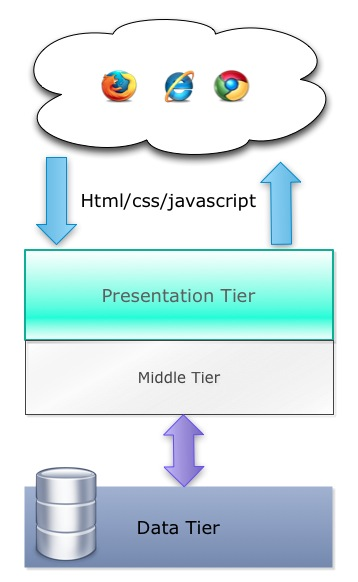
\includegraphics[width=0.48\textwidth]{images/architecture1.jpg}
 % \end{center}
 % \caption{Overal architecture 1.0}  \label{fig:architecture1}
%\end{wrapfigure}
%% FORTSETT
Architecture 1.0 is a backend-oriented Web app. All of the application's logic happens in a Web application that runs on an application server. In respect to \textit{Reference-model 1.0}, the application is separated into three software layers with different responsibilities; a presentation layer, a domain logic layer, and a data source layer. I have chosen this separation of concerns in order to facilitate application maintainability and flexibility. I could have chosen to implement everything in two, or even one layer, but this would resolve in classes having very many responsibilities, and possibly lots of code duplication. The layers cooperates by delegating responsibility. This means that the presentation layer implements client-server specific concerns, and delegates business logic specific operations to the domain logic layer. This layer implements business logic, and delegates to the datasource layer whenever it needs to address the database or some other data resource. The results from the operations done in the datasource layer bubbles up the layer stack all the way back to the presentation layer.

The Web app depends heavily on Http sessions to maintain user-state. When a user enters www.Shredhub.com, SpringMVC generates an object (called the HttpSession object) who's lifetime lasts throughout the user's session with the app. This object is used as a container for storing state information.

The application's front-end consists of a set of HTML pages that we will refer to as \textbf{Views}. The views are implemented with the JSP temple language technology, and are turned into HTML pages with the template view pattern. The client user primarily communicates with the app through three different interaction schemes: 
\begin{enumerate}
\item {} Links (anchor tags) 
\item{} HTML forms
\item{} Buttons or text input-fields that are picked up by JavaScript handlers
\end{enumerate}
For all of the different user-interaction schemes in listing 1 and 2, there will be a corresponding function (called a controller handler) on the backend. These actions always result in a new view being rendered and returned to the client. Interaction scheme 3 only occurs a few times on the app, in special cases that requires highly responsive behavior, in which a server round-trip must be avoided. This is managed by Ajax calls that are implemented in the views. 


In the following sections we will look into the implementation details of the source code. We will discuss the problems that occurred along the way, choices that were made, and potential alternative solutions. The discussion is divided into three; one part for each software layer in the application.

% \begin{figure}[h]
%  \centering
%  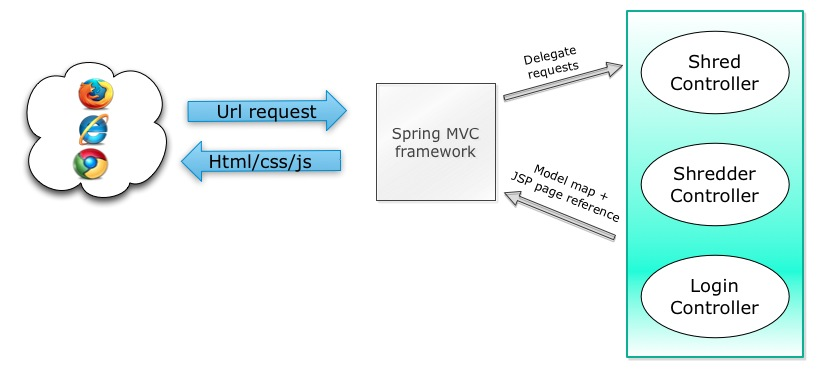
\includegraphics[scale=0.5]{images/presentationtier1.jpg}
%  \caption[sp.]
%   {The presentation tier's responsibility }
%    \label{fig:presentationtier1}
%\end{figure}
\section{The presentation layer}
The presentation layer is the first entry point in the application. Its responsibility is to handle client interactions, meaning it will handle authentication, session management, and input validation. The presentation layer is also responsible for knowing what operation to call in the domain logic layer, and it generates the views that are sent back to the client. It is built with the Model-View-Controller pattern, because this creates a nice and coherent separation of concerns. 

\subsection{Authentication}
The first entry point in a SpringMVC application is a set of interception filters. In Architecture 1.0 these filters are configured to handle authentication, access control and a bit of input validation. Users must to be authenticated in order to use any of the pages on Shredhub except the login page. Most of the authentication and access control handling is set up to be handled automatically by Spring, through the Spring security framework \cite{springsec}. Spring provides a lot of different authentication protocols, both based on standardized security protocols, and customized solutions made by third parties. For simplicity, I have chosen to use a Html form-based authentication mechanism that relies on a username, password and security-role. Other common authentication solutions used in Web apps are HTTP BASIC or HTTP Digest, or HTTP X.509 client certificate exchange. However, I find that form-based authentication fits the simple scope that has been chosen for authentication in this thesis, and it conforms to \textit{Reference-model 1.0}, because it relies on server's session handler.

The form based authentication process works by letting users enter a username and password in an HTML form on the login page. On form submit, the request is picked up by Spring's interception filters, which will look in the database for a Shredder with the given username, password. The database row for a Shredder also contains a column that represents the Shredder's user-security-role. However, for simplicity there is only one role in this app, which is the one that gives access to everything. If a row with a matching username and password is found, the framework will grant access to the user, and the user will now have access to the whole Web app. To avoid having to re-authenticate for every subsequent request, Spring will behind the scenes maintain a security-context object that is connected to the User's HttpSession. The security-context object simply indicates that the user has successfully logged in once, and is allowed to perform the given request. 
		  
\subsection{State Management}
In respect to \textit{Reference-model 1.0}, state is to be maintained on the server. 

The presentation layer is responsible for managing state associated with a User when he navigates around the app. In Architecture 1.0, this is implemented by using Spring's HttpSession object. The Spring IOC container creates one HttpSession object for every current User, which naturally is scoped at session-level. Considering that Spring offers readily available in-memory objects scoped at session-level, makes it very appropriate to use such objects as caches for data that is frequently accessed. In the Web app, I put state data either in objects that are maintained by the IOC container and scoped at session-level, or I put them directly on the HttpSession object, using a method called \textit{setAttribute(String key, Object value)}. The separation is a matter of separation of concerns; HttpSession object maintains meta data concerning the User (profile info, battle requests, battles, fanees etc), while other session-scoped objects maintains data regarding the User's page activities (e.g current shred-row, current shredder-page etc).

 Data that is used to populate views on the server has to be fetched from the database. Many of these database calls can be avoided if some of the data is stored in memory. The data could for instance be a particular set of Shreds that must be fetched especially quick in order to achieve responsive behavior, User data that is displayed often, e.g the User's name, or a list of battle requests which is meant to be visible on the top navigation-bar at all time. Shredhub needs to be very efficient and responsive, therefore solutions to avoiding repetitive and redundant database lookups has been prioritized in this architecture.The problem however, is that there is a tradeoff in how much data should be kept in memory, as maintaing too much memory might make the application slow, and in worst case lead to out of memory exceptions. Also, and this is a special case for typical Web 2.0 applications, data tend to change frequently, and users naturally want up-to-date views of the data. Hence, content regarding the Shreds and the newest Shredders on Shredhub, new fan-connections and other data that frequently changes, for simplicity shouldn't be cached. However, alternative solutions that makes it possible to cache such data is to some extend possible, for example by implementing push-based public-subscribe service that signals the cache to update whenever an update is made. Or alternatively a pull based solution where some service frequently pulls the database for new updates. A very simple proposal for such a solution is given later in this section.

Given below I have addressed two different collections of data objects that are frequently accessed in the application, together with an indication of how frequent the object changes, how often it is accessed, and the decision of wether they are cached in the User's session or not:
	
	\begin {enumerate}
	\item{} Data that is fetched in each Http request:
	
	\begin{tabularx}{\linewidth}{ | X  |l | l | l |}
	    \hline
	    \textbf{Data object} & \textbf{Changes}  & \textbf{Displayed} & \textbf{Cached in session}\\ \hline
	    The User's username &  Never & Always & Yes\\ \hline
	    The User's fanees & Moderate & Always & Yes\\ \hline
	    List of battle-requests for the User & Moderate & Always & Yes \\ \hline
	    The User's unique ID & Never & Always & Yes \\ \hline
	    \end{tabularx}
	
	\item{} Data that is accessed  frequently
	
	  \begin{center}
	\begin{tabularx}{\linewidth}{ | X  |l | l | l |}
	    \hline
	    \textbf{Data object} & \textbf{Changes} & \textbf{Displayed} & \textbf{Cached in session} \\ \hline
	    User's profile details, like address, guitars, age, email, birthdate, etc & Seldom & Moderate & Yes \\ \hline
	    The User's current battles & Moderate & Often & Yes \\ \hline
	    
	    The rows of Shreds that are displayed in the shred-pool & Often & Often & Partly \\ \hline
	    
	     Page navigation data, e.g page numbers and Shred-row numbers & Moderate & Often & Yes\\ \hline
	    The shred-news list & Often & Often & No\\ \hline

    	    Shred, Battle or Shredder the User just looked at & Moderate & Often & No\\ \hline
	   \end{tabularx}
	\end{center}
	
	\end{enumerate}	
	
In general, data objects that are frequently accessed and that is special to the User, should, and is being cached in the session. 

\paragraph{Table 1}:
 The reason I store everything in this table is because this data is accessed very frequently, it only addresses the User, and it doesn't change often. All of these objects are fetched when the User logs in, and for simplicity, I never pull the database for updates concerning this data. Hence, for instance if the User gets a new battle request during the session, it won't be visible until the next time he logs in. This is simply because I didn't have time to implement a pull/push based service, and I consider this behavior good enough for this thesis. 
 
\paragraph{Table 2}:
In the second table I have chosen to store the User's profile details, the User's current battles, and navigation data. The latter is just a set of small integer numbers that controls for example the page number for the list of Shredders the User is currently at, or which row number in a particular Shred-row on the shred-pool is the User currently at. This could also be stored in the Urls, however I chose to keep the Url's clean of state information, and instead maintain this state info on the server, as the Url option to a higher extend addresses \textit{reference-model 2.0}. The data objects mentioned here do not change very often, and are most likely small in size. These are also fetched when the User logs in, and aren't updated, unless update is made by the User himself. This could be for instance if the User updates his profile details, adds a new fanee or starts a new battle. In this case I eagerly write to the database, and at the same time update the cache.


The set of Shreds that are displayed in the shred-pool are only partly cached: the shred-pool is made up of multiple rows of Shreds. Each row consists of 3-5 Shreds, depending on which Shred-row it is, and the User can click a next button change the particular row to a new set of Shreds. Now, for each row, the server fetches a set of 20 Shreds from the database, and maintains these in a session-cache (or buffer). Whenever the User clicks on the ``next'' button in a row, the server checks the cache for that row to see if the next row of Shreds lies within the buffer. If they do, the row is moved one row-size, and this new row of Shreds are displayed. If not, the server fetches another 20 Shreds from the database and displays the first row from the new buffer. By using this buffer of Shreds for each row, the server avoids many calls to the server, which is very important in order to get quick and responsive behavior when the User clicks the next button. The buffer could also be bigger, but then again there is a tradeoff in how big the cache can be without influencing performance. 

The last two rows in table 2 concerns data that changes often and should always be up-to-date. In this case it is not worthwhile caching anything, considering the data must always be fetched eagerly from the database in order to be sure to have up-to-date data. The last row concern objects that could actually be saved in the cache, considering there is a chance the User might want to look at them again shortly, and in cases where the data is not likely to have been update yet. However, again, for simplicity I have chosen not to cache. 

\subsubsection{A Simple Cache Proposal}
As caching is very important for maintaining good performance , a simple caching solution for Shreds and other data that frequently changes is given in the following outline:
\textit{The caching scenario works by having a Java container object scoped at session-level, that maintains a HashMap of cached objects. The objects are be referenced by their database ID, so that whenever a request comes in for either a Shred, Battle or a Shredder object, the client of the cache container checks if the object with the Id is there. If so, it is returned, if not, the object is fetched from the database, put in the HashMap and returned to the requestor. To maintain updated values, there could be a background process that is triggered every time the cache is checked. For every object in the HashMap, the background process checks the database for the object with the given Id, and compares the value of the time-of-last-update field. If the object in the database has a newer time value, the database object is swapped with the outdated object in the cache. Spring provides many different implementations of an interface called TaskExecutor, which is able to perform background jobs both asynchronously and in concurrent fashions. An alternative to fire of the background job every time the cache is accessed is to use a Scheduled job that executes the background process every n seconds. } 

This cache could be used both for a User's session, such that data that concerns the user himself (for example the set of Shred, or Shredder recommendations that are displayed in the shred-pool ), or it could be maintained as a general cache for every user. This would maintain data that is frequently accessed by everyone, for example the list of the top rated Shreds that is displayed in the login page and in the shred-pool. Unfortunately I have not had the time to implement such a solution. 

It is worth mentioning that there are many alternatives for how data can be cached in memory in order to avoid consulting the database. Another approach I could have taken is to use a third party service like Memcached,\cite{memcached} which is a highly efficient in-memory storage of data that can be placed on the same machine as the application server, or (as recommended) distributed to multiple machines. This would extend the caching capability of Shredhub. Unfortunately, I did not have the time to integrate such a service for this thesis. 

\subsection{Input Validation}
Input validation is both part of the presentation layer, which addresses form-input rules, and the domain logic layer, which enforces business rules of the input data. In the presentation layer, validation is usually the first thing that happens once a Url request enters the server. Validation is always performed by applying positive filtering, meaning I specify what's allowed, and forbid everything else. Another approach is to do negative filtering where the input scanned for illegal patterns. However the latter approach is not as secure because it is hard to imagine all possible attack-forms.\cite{sqlinjection} Also, new forms of attacks might be invented in the future. However, positive filtering has the downside that it might be to restrictive.

Mainly I have two ways of verifying user input in the application. One of them is to enforce validation rules directly onto the variable in the domain object classes, I.e the Shredder class will contain validation rules concerning its data variables, the Shred class contains validation rules concerning its variables etc. This feature is something that's provided by Spring, using keywords in the domain classes that are automatically picked up by Spring. This validation is performed whenever the User creates a new domain object, such that the validation is executed before control is handed to a controller. The other way validation is done is by manually checking the Html form-input illegal input, or access rules. For example the controller often checks that the User stored in the session is allowed to perform a given business operation, or that a video file is sent when the User wants to add a new Shred. 

An example of validation rules applied to a domain object is displayed in the code below. This shows the use of regular expressions and other rules to define the format of the data that is allowed for a Shredder. The annotations (referenced by the ``@'' character) are picked up by SpringMVC whenever a new Shredder object is created. Spring will then check that the data entered matches the rules, if not, an error is generated. Hence positive filtering.
	
\begin{lstlisting}
	public class Shredder implements Serializable{
		
	        @Size(min=3, max=20, message=
	    		    "Username must be between 3 and 20 characters long.")
	     @Pattern(regexp="^[a-zA-Z0-9\\s]+$",
	     	message="Username must be alphanumeric")
	     private String username;
	     
	     @Pattern(regexp="[A-Za-z0-9._%+-]+@[A-Za-z0-9.-]+\\.[A-Za-z]{2,4}",
	    	        message="Invalid email address.")
	     private String email;
	     
	     @Size(min=6, max=20, message="Passwords must be between 6 and 20 characters long.")
	     @Pattern(regexp="^[a-zA-Z0-9\\s]+$",
	 	        message="Passwords must be alphanumeric")
	     private String password;     
	    
	     .... // other fields
	     
	     }
\end{lstlisting}
Before I went with this approach, I tried to implement negative filtering. Here, I created a custom validator class that would perform negative filtering on the user data. The validator's validation function is executed before the appropriate controller handler is called. The validator function would inspect the input to find potential illegal data. If any potential violation characters or patterns were found (for instance the sequence " ' OR 1=1; SELECT ...; -- ", which is a typical SQL-injection attack) I created an error message that is delivered to the controller function that is to execute next. This approach was very cumbersome, because it had to test for many different text patterns, and also, it is hard to know every possible set of illegal inputs.


\subsection{Controllers}
Controllers are first-class citizens in the presentation layer, who's responsible for processing URL requests. These components represents the Controller part of MVC. Controllers are Java classes that are mapped to specific a specific Url pattern. A simple approach is to have one controller class that is used for every Url supported by the Web app. However, this is not very maintainable, as the class would  grow exceptionally large, and have many responsibilities. Other solutions are for instance to have one controller class for every View, or one for every domain object. I have chosen to implement something in between. I chose to implement one controller class for each main resource/domain in the application, in addition to one controller for the login, and shredpool view (simply called the login controller). In the table below we can see all the controllers in Architecture 1.0, together with some example controller handlers and their respective responsibilities. Although not displayed in the table, note that each controller handler is mapped to a unique Url.

\begin{center}
    \begin{tabular}{ |  l  | p{6cm} |  l  |}
    \hline
	\textbf{Controller handler} & \textbf{Responsibility} & \textbf{View returned} \\ \hline    
    \multicolumn{3}{|c|}{HomeController} \\ \hline
    loginPage() & Handles requests for the login page. Fetches the top-rated Shreds from the database and renders the login page & The login view \\ \hline    
    
    loginSuccess() & Called when authenticating the User succeeds. Populates the session cache with data fetched from the database & None: redirects to www.shredhub.com/theshredpool \\ \hline
    
    theShredPool() & Fetches from the database the set of Shreds and all the shred-news that are to be displayed in the shred-pool. & The shred-pool view \\ \hline
    
      showShredInShredPool() & Given a Shred id, the Shred is fetched from the database and renders the shred-pool view so that it displays the Shred as a pop-up window on top of it & The shred-pool view \\ \hline
    
    \multicolumn{3}{|c|}{ShredController} \\  \hline
   
     createShred() & Creates a new Shred, saves to the database & The shred-pool \\ \hline

     postComment() & Ajax supported function that given a shredId and comment-text, adds a new comment to a Shred where the comment-owner is set to the id of the User (stored in session) & None \\ \hline
     
    \multicolumn{3}{|c|}{ShredderController} \\      \hline
getShredders() & Fetches the next page of 20 Shredders that are to be displayed in the list of Shredders view. The page number is maintained in the session object & The shredders view\\ \hline
followShredder() & Adds a new fanee to the User's list of fanees. Updates the session-cached list of fanees for the user  & The shredders view \\ \hline

newShredder() & Creates a new Shredder. Stores it in the database & The login view \\  \hline

 \multicolumn{3}{|c|}{BattleController} \\ \hline
 getBattle() & Fetches a battle object given a Battle Id & The battle view \\ \hline

newBattle() & Called when a Shredder accepts a Battle request that is being kept on the session object. Creates a new Battle object. Stores it in the database & The shred-pool view \\ \hline

getBattles() & Called when a Shredder accepts a Battle request that is being kept on the session object. Creates a new Battle object. Stores it in the database & The shred-pool view \\ \hline


    \end{tabular}
\end{center}

This controller granularity is very intuitive and coherent, and it makes it easy to extend the application with more actions. For example if I was to implement a new function for the application, say, the use case: ``remove a fanee-connection'', this would naturally be implemented as a new controller handler function inside the ShredderController class. I could however, have created even more fine-grained controllers, say a ShredPoolController, a FanController, or even a BattleRequestController, but I feel the amount of controllers fits the application quite well. 

\subsubsection{Control Flow}
In this section I will describe what happens in the controller when a Url request comes in. An example controller, and a controller handler is given in the code below. Extra comments are added to explain important things.
		
\begin{lstlisting}

// Handles all Url requests for www.shredhub.com/shredder*
@RequestMapping("/shredder")
@Controller
public class ShredderController {
		
	// Entrance to the domain logic layer
	@Autowired
	private ShredderService shredderService;
			
	// Handles a url requests for www.shredhub.com/shredder/<someFaneeId>/?action=follow
	@RequestMapping(value = "/{faneeId}", method = RequestMethod.POST, params = "action=follow")
	public String followShredder(@PathVariable int faneeId, Model model, HttpSession session) {
		Shredder user = (Shredder) session.getAttribute("user");
		List <Shredder> shreddersFanees = (List <Shredder>) session.getAttribute("fanees");
		try {
			
			// Delegate to the business operation
			List <Shredder> updatedFaneesList = shredderService.createFaneeRelation(user(), faneeId, shreddersFanees);
			
			// Update the session 
			session.setAttribute("fanees",updatedFaneesList);
			
			// Return the view that displays a list of 20 Shredders
			return this.getShreddersAndReturnShreddersView(model, session);
			
		} catch (IllegalShredderArgumentException e) {
			// Something wrong happened in the business operation. Return the error-page view
			model.addAttribute("errorMsg", e.getMessage());
			return "errorPage";
		}
	}}	  
\end{lstlisting}
This particular controller handler is triggered when the User clicks an anchor tag with the link given in the comment above. The shredderService reference is the gateway to the domain logic layer. SpringMVC's IOC container will inject a concrete implementation of ShredServices, because the pointer is annotated with an @Autowired field, which is picked up by Spring when the application is started. When the request comes in, the controller handler fetches the user from the session, because the business operation needs the User's Id and his corresponding list of fanees to check if the User is already a fan of the Shredder with id=<faneeid>. Note that if this Url request would be a form submit that contains user generated input data, the controller would first check the result of the input-validation process done by the interception-filters. If the validation process found en error, the controller handler return an error page immediately, instead of calling the logic layer. Anyhow, if a business operation is called, the controller would upon return catch any exception that might have occurred somewhere down the line. For example if the User is already a fan of the other Shredder. Note that I could have chosen to run this check inside the controller handler before I call the business operation, but this is strictly speaking a business rule that belongs in the business logic layer. If an error is found, the a Model object is populated with the data that is to be rendered together with the error view. The Model object represents the Model in MVC. This object will be used to contain the data that is injected into the views that are sent back to the user. Going further, if the business operation that was called succeeded, the controller calls a function that does the following:
\begin{enumerate}
\item{} Set p = the current page number stored in the HttpSession object
\item{} Ask the logic layer to fetch a list of 20 Shredders, starting from page num = p
\item{} Put the result list on the Model : model.addAttribute(``shreds'', resultList)
\item{} return the String ``shredders''
\end{enumerate}
The returning String is picked up by SpringMVC's View Resolver which I have configured to map my Java Strings to names of Jsp files. Hence the View Resolver will look for a view names ``shredders.jsp'', or ``errorPage.jsp'' in case the error view is returned from the handler. How the views are generated is explained in the next section. The reason I do this last part in a separate function is because it is called by other controller handlers as well. Also, the reason I chose to return the shredders page, is because it is from this page the User initially clicked the follow link, and therefore the controller just returns the same page as the user was in.
 
\subsection{Views}
Views represent the V of MVC. In Architecture 1.0, Views are implemented with the Java Server Pages (JSP) technology. JSP is fully supported by SpringMVC's template engine, and is a popular choice for dynamic view generation. The reason I chose JSP is because it has good support for many tag libraries, which extends the language features that can be used in the Views, and it makes it easy to integrate  the domain objects' data fields into the view. Also, it has a nice and intuitive syntax, that is more Java-like then other template technologies (for instance Velocity or Freemarker). However, one could argue that choosing Velocity or Freemarker is a better approach because its syntax is more appealing to non-Java developers. 

It is considered best practice to avoid implementing business logic in the views. \vref{Johnson04} View logic, on the other hand (code that generates the user interface), should only be done in the presentation layer, because it has got nothing to do with either the domain logic layer, or the datasource layer in terms of code-responsibility. To blend these responsibilities together would result in tight couplings between how the page looks like, and the data it operates on. This is one of the reasons I chose to implement the MVC pattern, because it nicely separates these concerns, making it easy to change the view without harming the business logic, and likewise to let the models be unaware of its presentation, so the presentation and models can change independently. Note that the models are implemented in the domain logic layer, but are used by controllers and views in the presentation layer.

\subsubsection{Main Components}
There is one View for each page in Shredhub. These are:
\begin{enumerate}
\item{} The login view
\item{} The shred-pool view
\item{} The shredders view
\item{} The shredder view
\item{} The Battle view
\end{enumerate}

Also, there are some views that are re-used in the above views:
\begin{enumerate}
\item{} the header view
\item{} the footer view
\item{} show shred view
\end{enumerate}

Each of these views are implemented as a jsp file, e.g login.jsp. The last three views in the list are injected into the other views using special JSP syntax, in order to avoid view duplication. The views contain static HTML tags that never changes, some Ajax functions written in JavaScript, and external links to CSS files and JavaScript libraries. JSP tags are used to inject the domain objects into the View by referencing to the Model object that is populated with data in the controllers. A simple example of the shredders view is displayed below:

\begin{lstlisting}[language=html]
<html>
<body>
	<jsp:include page="header.jsp" />	
	<h1>Shredders</h1>		
	<form action=``searchForShredder''>
		<p>Search for a Shredder </p>
		<input type="text"/>
	</form>
		
	<c:forEach items="${shredders}" var="shredder" varStatus="i">
		<div class="shredderInList">
			<img src="<c:url value="/resources/images/profiles/"/>$								{shredder.profileImagePath}"	alt="Profile img">

			<a href="<c:url value='/shredder/'/>${shredder.id}">${shredder.username}</a>
			<p>${shredder.description}</p>
			<p>Level: ${shredder.level}</p>
		</div>
	</c:forEach>
	<a href="<c:url value='/shredder/'/>nextPage">Next</a>
	<jsp:include page="footer.jsp" />
</body>
</html>
\end{lstlisting}
As we can see, the special template syntax is indicated with the ``<c:'' and ``$''. The c tags represents things like loops and conditionals, while the $ tag directly refers to objects that the controller handler has put on the Model object (as we saw previously). Here, we use a c:forEach to loop through a list of shredders that were given to us in the controller that returned this particular view. After a controller handler finishes, and the View Rendered gets this view together with a Model object, it compiles the view by executing the special JSP syntax, and outputs a fresh HTML page. SpringMVC sends the Html page back to the client. 
 
The next example shows the one and only place in the app where Ajax is used to implement dynamic in order to avoid fetching a complete view from the server. The example shows the a simplified version of how a Shred is displayed. Now, if the User rates or comments the Shred, the new result (I.e updated rating value or the new comment) has to be displayed very quickly in order to achieve proper responsive behavior. This could be solved the usual way by using form-submits, but in this case, this is not good enough, because it results in a complete page refresh in the browser. Everywhere else in the app however, regular form submits are ok.

\begin{lstlisting}[language=html]
	<srcipt type=``text/javascript''>
		function commentShred(shredId, commentText) {
			// Create the url that calls the controller handler on the server
			var baseUrl = "<c:url value='/shred/'/>" + shredId;
			var url = baseUrl + "/comment/?text=" + commentText;
	
			// Send the Ajax request to the server as a Http post request.
			// The result from the server is the Shred with the list of comments 
			// updated with the new comment 
			$.post(url,
			
			// This function is called when the server's response gets back
			function(shred) {				
				// get the last comment from the shred, I.e the one the User just created
				var lastComment = _.last(shred.shredComments); 
				
				// Create a comment as an html string,
				// that is to be injected into the DOM tree
				var htmlString = '<tr><td>' + lastComment.text + 
       			        '</td><td>' + lastComment.commenter.username + 
				'</td><td>' + new Date(lastComment.timeCreated).toUTCString() + '</td>'+
				'<td><button type="button" class="close"
				 onClick="deleteComment(' + last.id + ', ' + data.id + ');" >x</button></td></tr>'
				 
				 // Append the Html to the table of comments
				$('#commentTable tbody').append(htmlString);
			});
	}
	
	function rateShred(shredId, commentText) {
		// I have omitted the source code for this example,
		// But it's very similar to the function above
	}
</script>

	<div class="videoView">
		<video id="videoInModal" src=``<c:url value="/resources/videos/"/>''$										{shred.videoPath''</video>
			<p> Created at: ${shred.timeCreated} </p>
			<p">Number of raters:${shred.rating.numberOfRaters}</p>
			<p>Rating:${shred.rating.rating}</p>
			
			<p>Rate it:
			 <input type="range" id="rateValue" min="0" max="10" name="rating" value="5">
			<button id="rateButton"
				onclick="rateShred($('#rateValue').val()); return false;">
			Rate</button>
			
			<p>Write a comment</p>
			<input type="text">
			<button id="commentButton"
			onclick="commentShred($('#shredCommentText').val());
			 return false;">
			 Comment</button>
			
			<h3>Comments</h3>
			<table id="commentTable">
			<thead>
				<tr>
					<th>Text</th>
					<th>By</th>
					<th>At</th>
				</tr>
			</thead>
			<tbody>
				<c:forEach items="${currShred.shredComments}" var="c">
					<tr>
					<td> ${c.text} </td>
					<td> ${c.commenter.username} </td>
					<td> ${c.timeCreated} </td>
					</tr>
				</c:forEach>
			</tbody>
			</table>
	</div>
\end{lstlisting}

In order to display the video, I have chosen to use the HTML5 tag <video>. This tag makes the browser fetch the video from the Url defined in the ``src'' attribute of the video tag, display a video frame, and provide a play button that the User uses to start the video. Another alternative to show videos is by using streaming technology, where raw bytes are transferred in real time while the user watches the Shred. This way the whole video doesn't have to be fetched before it can start to play. However, the performance benefits with choosing either of these approaches is out of scope for this project, so I won't dig into it. 

Its worth noticing the \textit{onclick} attribute on the rate- and comment buttons. These are JavaScript handlers that are triggered when the user clicks either of the buttons. When the onClick events are fired, the browser will call a JavaScript function (one of the two we see in the code example) that uses Ajax to submit the request to the server. The result from the server is the updated Shred object which is used to populate manipulate the DOM tree to display the updated value. As stated in previous chapters, the JavaScript functions are independent, and self contained. An unfortunate property here is that the JSP view now contains Html, JSP tags and JavaScript. Three languages in the same file, which makes the code somewhat messy. I could put the JavaScript files in a separate source file, but the JavaScript would still have to use both Html and Jsp tags. 

\subsection{Summary of The Presentation Layer}
The presentation layer is built with MVC. Form submits and link actions are picked up by a specific controller handler on the server. The handler performs validation, state management, and delegates to a business function in the domain logic layer.

Models are implemented in a lower layer, but are heavily used by the presentation layer. After a business operation is performed, the Controllers are responsible for choosing which Model objects to send to a View, and the Views can access the data in the Model through special JSP syntax.

The presentation layer depends heavily on state implemented as session-scoped objects, but due to the nature of Web 2.0 applications, which requires data to have up-to-date values at all time, there isn't very much data to cache. Also, I acknowledged that there should have been a dedicated caching system in this architecture, but this was out of project scope to implement.
			
\section{The Domain Logic Layer}
The domain logic layer is the part of the application that receives a specific action from the controller, and performs the necessary business logic needed to complete the action. Now, since the responsibility of the logic layer is to implement the business logic in the application, it is important that this software layer is flexible. Flexibility, means that it can be relatively easy to add new features without harming anything else in the source code, and it should be easy to modify the already existing code. To achieve this, I needed a coherent design, preferably built with design patterns that gives a proper structure to the software architecture. To organize the layer, I have chosen to use the service layer design pattern \cite{poea}. This pattern creates a boundary into all of the application's business logic operations, by dividing the application into logical abstractions. Each abstraction represents the business operations that operates on a particular resource, or domain in Shredhub (e.g a Battle, a Shredder, or a Shred). However, this is not to be associated with the application's domain objects which concerns the domain resources' data, not functions. Instead, the service abstractions wraps the set of operations that are supported for each resource. Hence, each service class has a set of service functions. The list of service classes with some essential service functions are given below:
		\begin{enumerate}
			\item{} BattleService 
				\begin{itemize}
					\item{} getBattleWithId
					\item{} getOngoingBattlesForShredderWithId
					\item{} acceptBattleWithId
				\end{itemize}
			\item{} ShredderService
				\begin{itemize}
					\item{} addShredder
					\item{} getShredderWithId
				\end{itemize}	
			\item{} ShredNewsService
				\begin{itemize}
					\item{}getLatestShredNewsItems
				\end{itemize}
			\item{} ShredService
				\begin{itemize}
					\item{} getFanShreds
					\item{} getAllTags
					\item{} getShredsForShredderWithId
				\end{itemize}
		\end{enumerate}

\begin{figure}
		  \begin{center}
		\fbox{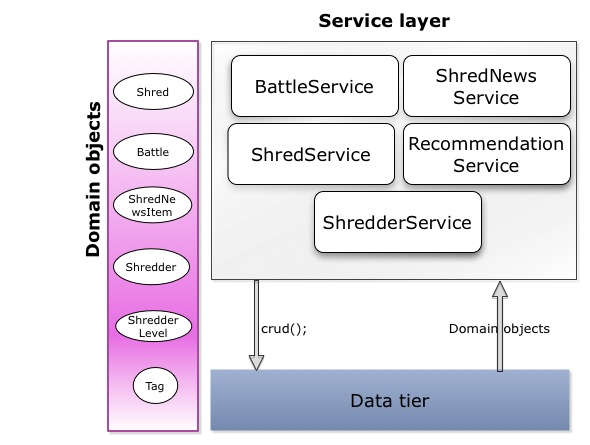
\includegraphics[width=14cm] {images/middletier.jpg}}
		% Kommandoen \fbox tegner en ramme.
		\end{center}
		\caption{The domain logic layer and its connection to the datasource layer}\label{fig:middletier}
\end{figure}

\subsection{Service Functions and Domain Objects} 
The service functions are called by the controllers in the presentation layer. An overview of the domain logic layer and its responsibility relative to the data source layer is given in figure \vref{fig:middletier}. The figure shows all the service abstractions, and the set of domain objects in Architecture 1.0. The domain objects represents the application's core resources, implemented as simple Java classes with no logical functionality, just attributes with accessor methods. The domain objects I have chosen to implement are Shred, Shredder, Battle and BattleShred. These objects have references to each other, and are used across all three layers in the application, making them the one means for communicating the domain in the application. The logic layer sends domain objects to the datasource layer in order to persist them. When the logic layer needs data from the datasource layer (e.g the database), the datasource layer will respond with domain objects.

An alternative architecture I could have chosen instead of the service layer pattern, is the table module pattern \cite{poea}. In the table module pattern,  all the SQL rows in the database gets a separate class that is responsible for performing the operations that are made on each row. However, this approach is very tight coupled to the database. Another alternative is to use the domain model pattern, which is often implemented in Ruby on Rails apps. Here, the domain objects would be responsible for performing business logic on themselves, and manipulate the database. This is a good approach, but the domain objects might end up being very big, with lots of responsibility. I prefer the solution of having a separate service class for each logical application abstraction, where the service functions performs all the necessary business logic for a given action, and the domain objects are plain data holders. However, a hybrid is also possible, where the domain objects implement parts of their logical behavior. However, I prefer to separate these concerns.
	
	
A final thing to point out is that because some service operations perform multiple  subsequent database transactions, each such service operation must be atomic. Spring achieves this behavior very elegantly by letting classes be declared as transactional, meaning every service operation in that class will be transactional (i.e have atomic behavior). In effect, if a database operation fails during a set of multiple database operations, the whole transaction is rolled back to the initial state. Hence atomicity (the A in ACID) is provided.  
	
\subsection{Data Flow}
Most operations in the domain layer follows the same structure; some data is fetched from the datasource layer, this data is manipulated together with the data it got from the calling controller handler, and the result is written back to the database. Also, sometimes the newly updated data is returned back to the controller, so that this can be rendered in a new view. If an error occurred along the way (for instance if illegal data was sent from the controller), an exception is thrown and picked up by the controller so it can return an error view. An example of a typical business operation is given in the code below:
	
	\begin{lstlisting}
	@Service
	@Transactional( readOnly=true )
	public class ShredServiceImpl implements ShredService {
	
		// Data source reference
		@Autowired
		private ShredDAO shredDAO;	
		
		/**
		* This adds a new rating to a Shred. 
		* When a shred is rated, the shred will gain a higher total rating, and
		* the shredder who made the shred also achieves
		* more experience points. Note that I don't check if the one who rates the 
		* Shred is the one who created it. This is a business rule that should be implemented
		* here, inside the business operation. However, for simplicity I have avoided it.
		*/
		@Transactional ( readOnly = false )
		public void rateShred(int shredId, int newRate) throws IllegalShredArgumentException {
			Shred shred = shredDAO.getShredById(shredId);
			if ( shred == null ) {
				throw new IllegalShredArgumentException("Shred with id: " + shredId + " does not exist");
			}
			if ( newRate < 0 || newRate > 10 ) {
				throw new IllegalShredArgumentException("Illegal rate value!");
			}
	
			// Here I could use the domain model pattern so that the
			// shred object itself knows how to set its own rating.
			// But I choose to follow the service layer pattern, where all the logic
			// is implemented in this service operation
			ShredRating currentRating = shred.getRating();
			currentRating.setNumberOfRaters(currentRating.getNumberOfRaters() + 1);
			currentRating.setCurrentRating(currentRating.getCurrentRating()+newRate);
			
			// store the result in the database
			shredDAO.persistRate(shredId, currentRating);		
			
			// Fetch the complete owner (Shredder) object from the database
			Shredder shredder = shredderDAO.getShredderById(shred.getOwner().getId());
			
			// Uses a utility class that is shared by all the service classes
			// in order to update the shredder level
			UpdateShredderLevel usl = new UpdateShredderLevel(shredder, newRate);
			usl.advanceXp();
			
			shredderDAO.persistShredder( shredder);
		}
	}
	\end{lstlisting}
This function is called by the controller handler that receives requests for adding a new shred rating. At first, it tries to fetch the Shred from the database, before it performs some input validation on the data it received. If all went well, the service function will set the new rating and persist the result back to the database. Then it will fetch the Shredder who initially created the Shred in order to increase the Shredder's experience points. Finally it will persist the Shredder back to the database. Note that just like the presentation layer did with the domain layer, the domain layer  delegates every persistency operation to the data source layer. The data source layer is reached through special references called DAOs. This is a nice separation of concerns, because the service functions only have to worry about the business rules, not how the data is persisted. Also, note that the operation in this example has to be atomic, because the function has multiple subsequent calls to the database. For example, if an error is made during the call to \textit{shredderDAO.persistShredder(shredder)}, the whole transaction will be rolled back to the state that was before \textit{rateShred} was called.

\subsection{Summary of The Domain Logic Layer}
The domain logic layer implements the domain of the application. The layer is divided into two; a service layer that implement business logic operations, and the domain objects which wraps the domain into self-contained data holders. The domain is divided into three abstractions; a Shred, Shredder, and a Battle class. The services are separated into a ShredService, ShredderService and BattleService class. The services forms a facade that is used by the controllers in the presentation layer. The services delegates to the data source layer for persistence.

	
\section{The Data Source Layer}
The datasource layer is the part of the application that receives a particular CRUD command from the domain logic layer, executes a SQL operation on the database, maps the result to a domain object and returns the result back to the business logic layer. I have chosen to use a PostgreSQL database, because it is open source, highly efficient, popular in the web industry, well documented, and most importantly, I know the database quite well. Also, I have chosen not to use an ORM mapping tool, but rather build Java functions that talks directly to the database using Strings as queries, and mapping query results manually to Java objects. There are many good ORM technologies I could have chosen to use, for example Hibernate, and JPA, which would hide the complexity of serializing Java objects to SQL, and the opposite, and not having to deal with SQL. However, these technologies does not give me the control I need to fine-tune, debug and create flexible and complex queries. A tradeoff though, is that writing SQL with java statements tend to get messy, especially when the queries gets many and complicated. I do however value the control one gets by explicitly writing every query with SQL. Obviously performance is important in this project, which makes it a big benefit to be able to take advantage of PostgreSQL's proprietary features.
		
\subsection{SQL Implementation}
The Java driver that connects to, and sends queries to the database is called JDBC. Spring provides a nice wrapper around the JDBC framework through a class named JDBCTemplate. This class takes care of all the boilerplate code like resource management and exception handling that is required when operating with JDBC. The SQL tables that represents the three central domain objects in the application is showed in the example below: 
		
\begin{lstlisting}[language=SQL]
	CREATE TABLE Shredder (
		Id				serial PRIMARY KEY, 
		Username		varchar(40) NOT NULL UNIQUE,
		BirthDate			date NOT NULL CHECK (BirthDate > '1900-01-01'),
		Email			varchar(50) NOT NULL UNIQUE,
		Password			varchar(10) NOT NULL
		Description		text,
		Address			text,
		TimeCreated		timestamp DEFAULT CURRENT_TIMESTAMP,
		ProfileImage		text,
		ExperiencePoints	int	DEFAULT (0),
		ShredderLevel		int DEFAULT (1),
		Guitars			text[],
		Equiptment		text[]
		
	);
	CREATE TABLE Shred (
		Id				serial PRIMARY KEY,
		Description		text,
		Owner			serial REFERENCES Shredder(Id),
		TimeCreated		timestamp DEFAULT CURRENT_TIMESTAMP,
		VideoPath		varchar(100) NOT NULL,
		ShredType		varchar(30) DEFAULT 'normal' CHECK (ShredType ='normal' or ShredType = 'battle')
	);	
	CREATE TABLE Battle (
		Id				serial PRIMARY KEY,
		Shredder1		serial REFERENCES Shredder(Id),
		Shredder2		serial REFERENCES Shredder(Id),
		TimeCreated		timestamp DEFAULT CURRENT_TIMESTAMP,
		BattleCategory		serial REFERENCES BattleCategory,
		Round			int DEFAULT 1,
		Status			varchar(30) DEFAULT 'awaiting' CHECK (Status ='accepted' or Status ='declined' or Status='awaiting');
	);	
\end{lstlisting}

In addition there are many-to-many relations between Shredders and Shreds, Shredders and Battles, and Battles and Shreds (actually BattleShreds, but they almost identical). Its important to mention them, because it requires the data source layer to perform complex join operations when fetching data from the database.

Now, there are lots of other smaller tables in addition to these, but these are the most essential. To perform the CRUD operations, I have chosen to structure my data tier around the Data Access Object (DAO) pattern. In this pattern, separate DAO objects are responsible for performing the relational data mapping on behalf of a particular domain object. This way the domain objects has no clue on how to persist themselves. An alternative to this is to use the Active record design pattern, where each domain object contains persistence code. However I prefer to keep this behavior separated from the domain objects as they would grow quite large and complex if they where to contain all the necessary object relational mapping code. Figure \vref{fig:datatier}
	\begin{figure}
	  \begin{center}
	    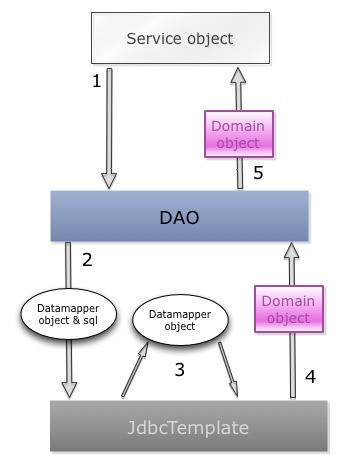
\includegraphics[width=0.5\textwidth]{images/datatier.jpg}
	  \end{center}
	  \caption{Data access pattern in the data tier}  \label{fig:datatier}
	\end{figure} 
	shows how object relational mapping is done in the data tier. Here's what happens when the domain logic layer asks the datasource layer to perform a CRUD operation (e.g a Read operation).
		
\begin{enumerate}
\item{} The logic layer calls a persistence function on a particular DAO object, for instance \textit{shredDAO.getShredById(int shredId); }
\item{} The DAO class uses a JDBCTemplate instance (injected by the Spring IOC container) to delegate the boilerplate behavior, for example getting a database connection. The JDBCTemplate is also responsible for executing the database query itself, provided that it gets a SQL statement from its caller. For instance: 
	\begin{lstlisting}
	@Service
	public class ShredDAOImpl implements ShredDAO {
	
		@Autowired
		private JdbcTemplate jdbcTemplate;
		
		public Shred getShredById(int shredId) {
			String sql =  "SELECT * FROM Shred s,Shredder sr WHERE s.Owner = sr.Id AND s.Id = ?";
			return jdbcTemplate.queryForObject(sql, new Object[]{shredId}, new ShredMapper());
		}
	}
	
	\end{lstlisting}
\item{} The JDBCTemplate is built with the template method design pattern, meaning it does callbacks to a mapper object provided by the caller. In the above code, the callback calls a function in the ShredMapper class. This class knows how to build a Shred object given the result from a database query that the JDBCTemplate executes. An example of how a ShredMapper class might look like is given below:
Example:
\begin{lstlisting}
public class ShredMapper implements RowMapper <Shred>{
	
	public Shred mapRow(ResultSet rs, int rowNum) throws SQLException {
		Shred shred = this.setConcreteShredder();
		shred.setId(rs.getInt("id"));
		shred.setDescription(rs.getString("Description"));
		shred.setOwner( new ShredderMapper().mapRow(rs, rowNum) );
		// Another template method!
		this.addConcreteBehavior(rs, shred, rowNum);
		return shred;
	}
}

\end{lstlisting}
Notice that I also use the template method pattern to enable customized mapper functionality that can be overridden by subclasses of the ShredMapper class. This is done with the BattleShredMapper, which extends the ShredMapper class, and hence overrides setConcreteShredder() and addConcreteBehavior(). 
	
\item{} The domain object created by the mapper is returned from the JDBCTempate back to the DAO object, which depending on the type of query might catch an exception to provide nice feedback to the service function. An example might be thrown by the DAO if a Shred with the given Id does not exist.
\item{} Finally the DAO function returns the domain object back to the middle tier. 
\end{enumerate}	
	
\subsection{Storing Video Files}
Media content is a central part of the application, since the primary purpose in the application is to share videos of people playing guitar. The videos have a maximum size of (x) bytes, because Shreds are supposed to be short (less then one minute). If a user tries to upload a file that is bigger then this, then an error message is given to the user. 
	As mentioned in the presentation layer section, the whole video is downloaded to the clients web browser before it can be played. It is therefore important to offer efficient uploading speed from the application's backend. As for now, I store the videos locally on the machine that is hosting the application, inside a folder that is publicly available for the users. This has some unfortunate drawbacks. One is that the users can directly access which ever files they want on the server, if they know the url for the video. The path to where the video's are stored can be seen if one inspects the HTML source code that is sent to the client's browser. The user could simply guess the name for a movie, and try to fetch it from the server. A second problem by having no protection of the videos is that it would be easy to do overflow attacks, where an attacker simply asks for a whole lot of videos until the server breaks down. A third problem is that storing the files on the machine that hosts the server requires a lot of storage space on that particular deployment server. This is undesirable, because one would not want to waste deployment space on something that could easily be stored elsewhere. Therefore I have explored various ways to store the media content, that is not being on the deployment space. One good example is storing the videos and images on  Amazon ec3 cloud storage. This is service is free of charge up to some x amount of requests and y amounts of data. There are also other alternatives to amazon, like SimpleCDN and windows azure, and they all look very similar in both pricing and performance. Unfortunately, I have decided that this is simply too time consuming to set up for this thesis, and therefore I have had to content myself with the simple solution described in the beginning of this section.
	
\subsection{How Much Data to Fetch}
Another issue is the challenge with deciding how much data to fetch from the database when an object is requested. For instance when a request is made for a Shred, should the DAO function fetch the whole Shred object, fetch the Shred's owner, all the tag objects for the shred, all the comments and rating etc. This is a tradeoff decision, considering fetching everything requires many SQL joins and much data-mapper processing in Java. But it avoids having to fetch the server for more data at a later point in time, if more of the domain object has to be fetched. One approach is to eagerly fetch every table column and to populate every foreign reference, which would require a large amount of processing, very much data stored in memory, and much data returned back to the client that probably will never be used. The decision I have made is to implement CRUD operations that are customized for the controller handlers in the presentation layer. For example, if a list of shredders is needed that are to be displayed in the shredders view, the read operation called in the database will populate a list of Shredders without their related list of fanees, shreds and battles. This is because these lists aren't needed in the Shredders view. On the other hand, if the shredder view is to be rendered, the database will populate the Shredder with all its fanees and all its shreds.		

\section{Summary of The Data Source Layer }
The data source layer is responsible for manipulating the database. The database is built with PostgreSQL, where object relational mapping is manually built in Java using, instead of using an ORM tool. This requires a lot of Java code, but, being built with design patterns like the DAO-, and template method pattern, the code is very flexible and facilitates optimized object mapping and querying.      


\section{Summary}
Architecture 1.0 is a Java web app built with SpringMVC. All the application's logic happens on the server, where the code is divided into three separate layers; the presentation-, domain logic- and datasource layer. The presentation layer is built with the MVC pattern, in which controller handlers handles Http requests, calls a business operation in the logic layer, and upon return, populates a Model object with data that is needed to create a View that is rendered to an Html page and sent back to the user. The domain logic layer implements business operations, and delegates the persistency handling code to the datasource layer. The application relies heavily on the Session object to maintain state. 
		
